\chapter{Choice of Engine}

\todo{Introduce the purpose and (weight) of the game engine analysis chapter - Endre}

\section{Introduction}
We where asked to analyse different game engines by the Norwegian Train Driver Academy, \textit{\Gls{lokforerskolen}}, since they have plans to migrate their existing simulator\footnotemark[1], which was created in \textit{\gls{jmonkeyengine}}, to another game engine. This change is mainly scheduled to prevent the risk of using an engine that no longer gets maintained or updated. To help them make this transition smoother, we have compared and analyzed different modern engines that is available today, and will give an answer as to which engine we believe fits their requirements best.

It was a requirement by \Gls{lokforerskolen} to include \Gls{unity} and \Gls{unrealengine} in the analysis, while \Gls{godot}, \Gls{open3dengine} and \Gls{cryengine} were additionally chosen based on their usage within game development.\cite{g2_game_engines_comp}
We compared the game engines based on both the absolute and desired functionalities set by \Gls{lokforerskolen}, code languages, expected learning curve for each engine and feedback from developers that has worked with each of the engines. 

\footnotetext[1]{Lokførerskolen's current simulator: \url{https://lokforerskolen.no/aktuelt/simulatorsenteret/}}


\subsection{Thesis Statement}
The increasing obsolescence of \textit{\gls{jmonkeyengine}}, a game engine used by The Norwegian Train Driver Academy, motivates the migration of their educational train simulator to a modern game engine. To identify and decide upon a future-proof game engine, the functionality and relevancy of several engines must be analysed and compared.


%%%         UNITY           %%%
\subsection{\Gls{unity}} 
The game engine was released by Unity Technologies in 2005 as a Mac OS-exclusive software, but has later granted support for a variety of platforms including web, mobile, console and virtual reality. \Gls{unity} proves itself as a capable engine and displays its wide range through games such as the mobile hits \textit{Pokémon Go} and \textit{Call of Duty: Mobile}, and large-scale games such as \textit{Cities: Skylines} and \textit{Escape From Tarkov}.

Today, the engine is notorious for its ease-of-use and popularity among indie developers \cite{unity_dealessandri_2020}, and is commonly described as an effective and efficient platform.  \cite{stepico_games_2021} It is no secret that Unity is a popular engine, with their CEO John Riccitiello claiming the engine is behind 60 to 70 percent of all extended reality\footnotemark[1] applications. \cite{chaudry_2020}

\footnotetext[1]{Abbreviated as \textit{\acrshort{xr}}. Term referring to alternate reality mediums, including virtual reality (\acrshort{vr}) and augmented reality (\acrshort{ar}).}

The \Gls{unity} license model\footnotemark[2] is split into Personal, Plus, Pro and Enterprise. Their Personal license makes the engine free to use if the annual revenue is below \$100,000. If revenue exceeds \$100,000, their Plus license applies, starting at \$40 per month. Should annual revenue exceed \$200,000, you are required to use the Pro or Enterprise plans, costing \$150 and \$200 per month, respectively. 

\footnotetext[2]{Unity license model: \url{https://store.unity.com/compare-plans}}


%%%           UNREAL           %%%
\subsection{\Gls{unrealengine}}
Created by Tim Sweeney in 1998, \Gls{unrealengine} was initially used during the development of the first person shooter Unreal. It was designed for fast-paced, multiplayer shooters, but has opened up to a wider audience after its public release. Today, the engine is maintained by \textit{Epic Games}, the developers behind large-scale games such as \textit{Fortnite} and \textit{Gears of War}, contributing to show off the engine's capabilities. It is known in the industry for its photo-realistic graphics, lighting, and advanced functionality such as ray tracing and advanced physics. The engine's full source code is written in C\texttt{++} and is available on \Gls{github}\footnotemark[1].

\Gls{unrealengine} offers two standard licenses\footnotemark[2] for different uses, the Publishing License and Creators License. The Publishing License allows for games and other off-the-shelf interactive products to be sold, but with a 5\% royalty after \$1 million in sales revenue. The Creators License has no royalties, but is for internal, non-commercial, or custom applications. \cite{unreal_licence}

\footnotetext[1]{Unreal Engine source code: \url{https://www.unrealengine.com/en-US/ue4-on-github}}
\footnotetext[2]{Unreal Engine license model: \url{https://www.unrealengine.com/en-US/download}}


%%%           GODOT           %%%
\subsection{\Gls{godot}}
Development of \Gls{godot} started in 2007 by Juan Linietsky and Ariel Manzur. The first release of the engine was in 2014. The engine was created because of the the technological progress of hardware devices that the engine present at that time did not account for. \cite{waiting_for_vr_2016} There are no large-scale games created with \Gls{godot} yet. The majority of games created are by small indie teams with restricted budgets.

Today, the engine focuses on their new release of \Gls{godot}; version 4. They are working on improving their own \acrshort{api}, adding Vulkan's graphics \acrshort{api} and other features to improve the engines overall performance. \cite{godot_improvements_verschelde_2022} \\

The engine is published under the \acrshort{mit} license making it free to use for any purpose. \cite{godot:licence} It is community driven and allows anyone to contribute to the engine source code. \cite{godot_introduction}

%%%         Open 3D Engine         %%%
\subsection{Open 3D Engine}

Open 3D Engine is the successor to Amazon Lumberyard, which itself is based on CryEngine. The initial version of the engine was released on July 6, 2021. Maintained by the Open 3D Foundation, an open source, umbrella organization under the Linux Foundation. \cite{open3d_foundation} 

The engine is open source, and there are no fees or royalties for using the engine. It is licensed under Apache 2.0. \cite{open3d_licence}

Given Open 3D Engine is the successor to Amazon Lumberyard, which featured VR support, we expected Open 3D Engine to also have VR capabilities. However, this seems to not be the case, as VR support is not included in Open 3D Engine. As VR is an absolute requirement for this task, this eliminates the engine from further analysis. 


% -----------------------------------------------------------------------------------------------%
%%%         Absolute Requirements           %%%
\section{Absolute Requirements} \label{absoluterequirements}

All of the engines analysed has support for 3D and virtual reality development, with the exception of Open 3D Engine not supporting VR. All engines has the capability to deploy the application on a Windows operating system. Input detection is supported by all engines as long as Windows detects and recognizes the device. The following table consist of each engine's status for the absolute requirements set by Lokførerskolen.

\begin{table}[H]
    \footnotesize
    \centering
    \begin{tblr}{
      colspec={|X[0.13, l]|X[0.17, l]|X[0.21, l]|X[0.17, l]|X[0.17, l]|X[0.15, l]|}, hlines,
    }
       & \textbf{Unity} & \textbf{Unreal Engine} & \textbf{CryEngine} & \textbf{Godot} & \textbf{Open 3D Engine}  \\
        \textbf{VR support} & Yes, with official plugin \cite{technologies_2022} & Yes & Yes, requires manual setup, workflow can be tedious\footnotemark[1] & Yes, but not as extensive & No \\
        \textbf{3D support} & Made for 3D and 2D & Only supports 3D & Made for 3D & Yes, but better suited for 2D \cite{godot_dealessandri_2020} & Yes  \\
        \textbf{Windows support} & Yes & Yes & Yes & Yes & Yes  \\
        \textbf{External input support} & Handled in-engine, and can be mapped in the editor & Handled in-engine, and can be mapped in the editor & Yes, but requires manual set-up through code & Uses universal input mapping, advanced input can be challenging & Yes, but requires manual mapping with C\texttt{++} \\
        \textbf{Modernity} & Continually updated, has a large and active community & Active development, Unreal 5 in early access. Internal tools used by Epic Games are often made public  \cite{unreal_5_early_access} & Has planned further development where developers are involved in the process \cite{cryengine_roadmap_2021} & Community driven and independent development. Does not rely on sponsor opinion, only developers. & Community driven and future-oriented \\
    \end{tblr}
    \caption{Table of absolute requirements for game engine features}
\end{table}

Technological progress has a major factor when considering if engines can reproduce any functionality. We have to take Lokførerskolen's claim that jMonkeyEngine is obsolete into consideration. The probability of migrating any physics, user interface or other functionality into a modern engine is high due to better, more updated features. 

\footnotetext[1]{Unlike the other engines, CryEngine requires rebooting in VR-mode for testing. \url{https://docs.cryengine.com/display/CEMANUAL/Oculus+Rift}}


%--------------------------------------------------------%


%%%         Desired Requirements        %%%
\section{Desired Requirements}
Lokførerskolen stated a desire to reuse the assets from their current simulator. The 3D file types currently used are Graphics Language Transmission Format (\texttt{.gltf}), AC3D Files (\texttt{.ac}) and Standard 3D Image Format (\texttt{.obj}). The present audio formats are Waveform Audio File Format (\texttt{.wav}) and MPEG-1 Audio Layer 3 (\texttt{.mp3}). The 3D file types are prioritized higher than the audio files because they would be more time consuming to convert or recreate. Of the 3D file types it is the \texttt{gltf}-files that are the most prioritized because of it's quantity in the current simulator.

\begin{table}[H]
    \centering
    \begin{tblr}{
      colspec={|X[0.16, c]|X[0.16, c]|X[0.30, c]|X[0.22, c]|X[0.16, c]|}, hlines,
      cell{2}{2} = {red9}, cell{2}{3} = {yellow9}, cell{2}{4} = {red9}, cell{2}{5} = {green9},
      cell{3}{2} = {red9}, cell{3}{3} = {red9}, cell{3}{4} = {red9}, cell{3}{5} = {red9},
      cell{4}{2} = {green9}, cell{4}{3} = {green9}, cell{4}{4} = {red9}, cell{4}{5} = {green9},
      cell{5}{2} = {green9}, cell{5}{3} = {green9}, cell{5}{4} = {green9}, cell{5}{5} = {green9},
      cell{6}{2} = {green9}, cell{6}{3} = {red9}, cell{6}{4} = {red9}, cell{6}{5} = {green9},
    }
      %\textbf{File Support}
      %\theadset\theadfont\backslashbox[25mm]{ \\File type}{Engine}
      & \textbf{Unity}\cite{unity_supported_files_2021} & 
      \textbf{Unreal Engine}\cite{unreal_supported_files} & \textbf{CryEngine}\cite{cryengine_supported_files_haan_2019}  & \textbf{Godot}\cite{godot_supported_files_lovato_2020}  \\
        \textbf{glTF} & No & Experimental & No & Yes  \\
        \textbf{ac} & No & No & No & No \\
        \textbf{obj} & Yes & Yes & No & Yes \\
        \textbf{wav} & Yes & Yes & Yes & Yes \\
        \textbf{mp3} & Yes & No & No & Yes \\
    \end{tblr}
    \caption{A matrix of file support for each engine}
\end{table}

%------------------------------------------------------%


%%%         Code Language       %%%
\subsection{Code Languages}
\subsubsection{C\texttt{\#}} \label{csharp}
This compiled language, developed and maintained by Microsoft, is the only officially supported programming language of Unity. \cite{unity_technologies_2021} It is also supported as an optional language for Godot and CryEngine. Similarly to Java, the language has features like automatic garbage collection, high-level syntax, and being a object-oriented language.

 C\texttt{\#} is used either natively or optionally in several game engines, making it a good choice as it gives the opportunity to change game engine without having to learn new code languages, only new engine specific features in combination with the code language.

\subsubsection{C\texttt{++}} \label{cpp}
C\texttt{++} is a low-level language and an extension of C. It is known for its performance, flexibility and efficiency. 
All of the four compared engines are written in C\texttt{++}, while Unreal Engine and CryEngine also use the language for scripting game logic.

C\texttt{++} is widely considered the gold standard in game programming \cite{terziyan_2020}, and has been used for blockbuster games such as \textit{Counter-Strike} and \textit{World of Warcraft}. Its object-oriented style and manual memory management contributes to emphasize good code practises and game development strategies such as design patterns and optimization. When used correctly, the statically typed language boasts a performance and efficiency unlike any of the other candidates. Working in close proximity to the hardware offers precise control over the environment, yet also introduces room for human error. 

Unreal Engine refers to its C\texttt{++} as \textit{assisted C\texttt{++}} due to offering features such as class wizard which sets up a class from scratch or a garbage collector for all classes. Unreal also provides ways for Blueprints (\ref{unreal:blueprints}) and C\texttt{++} code to work together.
\cite{unreal_engine_documentation_2021}

\subsubsection{GDScript} \label{subsubsec:gds}
GDScript is an interpreted scripting language, meaning it gets interpreted at run-time. It benefits when the program requires the code to be platform independent, dynamically typed, and have a small executable size. GDScript is similar to Python in the way that individual blocks are indented and many of the keywords are similar. The language was created to be integrated and optimized with the Godot Engine. \cite{gdscript_basic} Choosing GDScript over Godot's alternate language C\texttt{\#}, results in up to four times slower performance. \cite{godot_engine_c_sharp} 



\subsection{Visual Scripting}

\textbf{Unreal Blueprints} \label{unreal:blueprints}

The Blueprint system in Unreal is flexible and powerful, as it allows the same concepts, logic and tools only available to programmers to be used by non-programmers. Blueprints and code can be integrated with each other, and blueprints should often extend the functionality of baseline systems created by programmers. There are several types of blueprints for different use cases, such as the “standard” Blueprint Class and the Level Blueprint which acts like a global event graph on a level, among others. \cite{unreal_blueprint_overview} Its ability to do almost everything C\texttt{++} can in terms of scripting, means it is the most robust and powerful visual scripting system of the engines in this comparison.

\textbf{Unity Visual Scripting} \label{unity:visual_scripting}


Unity's Visual Scripting system is quite new, and has been included since version \texttt{2021.1}. Earlier versions of the engine requires Bolt Visual Scripting, an external package, to enable visual scripting. Bolt started as a community project, but was acquired by Unity to be integrated as the official visual scripting system. \cite{unity_aquire_bolt} Visual scripts can be divided in two main categories, Flow Graphs and State Graphs. \cite{unity_visual_scripting} In order to use a visual script on a GameObject, a Script Machine component is added, which can hold a Visual Script asset. This process decouples the script from the machine. Visual scripts can be integrated with and use code, events and properties from the engine, third party plugins and custom scripts. \cite{unity_visual_scripting_docs}

\textbf{CryEngine Flow Graph} \label{cryengine:flow_graph}

Flow Graph is CryEngine's main visual scripting tool. Its main uses include creating mission logic and controlling entities and AI in a level. Flow Graph is also used to prototype sound design, effects, and gameplay, as they allow rapid iteration compared to code. 

Schematyc is a beta feature in CryEngine. It is designed to control objects in a level, while Flow Graph is more geared towards scripting for the entire level and mission. Another important design aspect is latency, determination and synchronization, with a more distinct execution flow between nodes of different types. Due to the beta status of this feature, it is not ready for production level projects, and should only be used in test projects. \cite{cryengine_schematyc}

\textbf{Godot VisualScript} \label{godot:visualscript}

VisualScript in Godot is more closely related to GDScript in terms of setup and functionality, compared to other visual scripting tools. Visual scripts are attached to game objects the same way other scripts are, and provides one graph per function. \cite{godot_visual_script_tutorial} Because the Godot Engine API is the same across different script languages, and the library for VisualScript needs improvements, there seems to be little to no benefit to using VisualScript.

%---------------------------------------------------%


%%%             Learning Curve                  %%%
\section{Learning Curve}

A learning curve is often used to present the relationship between someones proficiency and experience for a task. In this section, we will analyze and discuss the game engines and their learning curves to form a holistic understanding of their steepness. To compare the learning curves, we have chosen to review specific aspects we believe will be of great importance for this project.

\begin{wraptable}{r}[0cm]{4cm}
    %\centering
    \captionsetup{font=footnotesize}
    \begin{tblr}{ | l | l | } 
      \hline
      \textbf{Engine} & \textbf{Score} \\ 
      \hline
      Unity & 8.5 \\ 
      \hline
      Godot & 8.2\footnotemark[2] \\ 
      \hline
      CryEngine & 7.9\footnotemark[2] \\ 
      \hline
      Unreal Engine & 7.4\footnotemark[2] \\ 
      \hline
    \end{tblr}
    \caption{Scoring by G2}
    \label{table:g2scoring}
\end{wraptable}
\bigskip
G2, the world's largest marketplace for reviewing software\footnotemark[1], have ranked the four engines' ease of use from 1 to 10, based on reviews from users. These ratings from G2's data \cite{g2_game_engines}, are as shown in \ref{table:g2scoring}.

\footnotetext[1]{G2: \url{http://company.g2.com/about}}
\footnotetext[2]{Disclaimer: The rating may be inaccurate due to an insufficient amount of reviews for this engine.}

\subsection{Documentation}
Software documentation should be structured, concise and contain explanations, examples and tutorials to trivial features everyone will encounter when developing in an engine. The engine documentations are set up as tree structures, branching into pages containing smaller topics, using hyperlinks to navigate to the desired page.

However, navigation isn't the only factor regarding ease of use for documentation. The intuitiveness of the documentation structure also impacts the ease of use. The Information Architecture Institute defines information architecture as “The art and science of organizing and labeling web sites, intranets, online communities and software to support usability and findability”. \cite{what_is_ia_IA_institute} With this definition, both Unreal Engine and Unity scores high because their layout of preview images provides a clear overview of the contents. CryEngine and Godot's respective documentation does not emphasize findability to the same degree.


As a proof of concept, we tried to find the documentation page for virtual reality in each engine's documentation, measuring the ease of use based on perception and intuition. For Unity, the reference to VR is found in the main page of the documentation. It contains how to get started, a pre-made VR template and links to other relevant material. Meanwhile in Unreal Engine, the information for VR was found in a subsection from the documentation main page. The information found in the section was start-up guides and best practises for each of the supported headsets. In CryEngine's documentation, the VR section was located in the main page. There was information on how to use the functionality, but no structured guide or additional information. In Godot, the VR section is exposed on the main page, but further navigation lacked intuitiveness for where to find a start up-guide and general documentation. 



\subsection{Community Support}
All of the engines have some sort of community support, with either forums, tutorials or community platforms. Unity and Unreal Engine has the biggest community among the four due to their popularity and use in the industry \cite{buckley_2022}, where Unity is usually biggest within indie games while Unreal is better suited for larger scale games. \cite{evercast}
CryEngine has a smaller community compared to Unity and Unreal Engine, making it difficult to find solutions for related issues. There is also less community created resources to learn from. Although its lack in size could make it easier to come in contact with the developers. \cite{cryengine_dealessandri_2020}
Godot is very similar to CryEngine in the sense that it has a small community compared to Unity and Unreal Engine. 
\cite{godot_dealessandri_2020}

\subsection{Development Tools}
All four engines include tools for editing materials. Unreal Engine, Unity and Godot have the option to use a graph-based approach for editing materials from the included editor features. CryEngine is limited to a drop-down menu for editing materials.

Source code access lets developers change the code on which the engine is built. This comes in hand when the developers wants to make noticeable changes to the physics or other engine attributes. All of the engines offers their source code to be viewed for free except Unity which requires the enterprise licence.

The only engine that offers VR editing mode is Unreal Engine, this is an approach to game development which allows the developer to virtually edit games. \cite{Unreal_VR_mode}

Unreal Engine and Unity offers dynamic occlusion culling \footnotemark[1] \footnotemark[2], a trait of the rendering pipeline deciding which game objects to exclude from the draw call at runtime. This saves the graphics processor from drawing any vertices not seen by the player, offering a great boost in performance.

\footnotetext[1]{\url{https://docs.unity3d.com/Manual/OcclusionCulling.html}}
\footnotetext[2]{\url{https://docs.unrealengine.com/4.27/en-US/RenderingAndGraphics/VisibilityCulling/}}

In CryEngine, the culling is done by the graphics API, ignoring vertices not seen on the final screen, although this gets done by default in all engines. Engine-level culling would need manual setup. Godot's occlusion culling requires manually specifying which objects to be ignored by the draw call. 

Both Unreal Engine, CryEngine and Godot have integrated tools for generating splines called Blueprint Splines\footnotemark[4], Spline Distributor\footnotemark[5] and Path\footnotemark[6], respectively. These tools generate curved paths based on set points in the engine's world-space, which can be useful for generating train tracks. Unity has similar features through the official package \textit{ProBuilder}.

\footnotetext[4]{\url{https://docs.unrealengine.com/4.27/en-US/BuildingWorlds/BlueprintSplines/}}
\footnotetext[5]{\url{https://docs.cryengine.com/display/CEMANUAL/Spline+Distributor}}
\footnotetext[6]{\url{https://docs.godotengine.org/en/stable/classes/class_path.html}}

\subsection{Scripting}
The considered programming languages, disregarding visual scripting, have an established order of difficulty. 

GDScript's resemblance to Python, a language well-known for being one of the easiest to learn, makes it a strong candidate for the simplest coding language. It is adequate for beginners due to being dynamically typed and syntactically friendly. To add code logic in Godot, simply add a script to a game object, which generates a script template. Granted Godot becomes our engine of choice, the choice of GDScript as the development language is not certain, due to  C\texttt{\#}'s advantages (\ref{subsubsec:gds}). 

Similarly, in Unity, C\texttt{\#}-scripts are added as components to tell game objects how to behave. The user can define the order of execution by implementing event callbacks such as \textit{Start} and \textit{Update}, while the engine handles the code execution loop. Unity offers several official code libraries for concepts such as math, physics and debugging, to support the development. 

Despite having a steeper learning curve, C\texttt{++} has become an industry standard for high-end game development. As if the language itself wasn't hard enough to grasp, CryEngine requires manually setting up the code framework, separating the code from the engine, and has an insufficient amount of learning resources due to the engine's low popularity. Scripting game logic works similarly to Unity and Godot, where scripts are added to entities.

Due to the similarity to Java, and features mentioned in C\texttt{\#}(\ref{csharp}), the transition from Java to C\texttt{\#} should be straightforward.   

C\texttt{++} is the main scripting language of Unreal Engine. The engine's base building block is called \textit{UObject}, and is used by the \textit{AActor} class, among others. The lifecycle of an AActor starts with \textit{BeginPlay}, an event which is called when the actor is first spawned into the game world. It then goes into the Tick life cycle, which is called once per frame until \textit{EndPlay} is called when the AActor leaves the world. \cite{unreal_engine_documentation_2021}. Due to the complex functionality stated in C\texttt{++}(\ref{cpp}), the language is commonly defined as one of the more difficult languages to learn as a beginner.

%--------------------------------------------------------%


%%%             Existing Solution          %%%
\section{Existing Solutions}

To gather insight from the industry, we contacted developers behind relevant games and simulators. The process included finding games made in the applicable engines, determining their relevance to trains, simulation or virtual reality, and contacting their studio/author by email. All subjects agreed to having their answers cited as part of our thesis.

When asked which engine they believe is best suited for VR game development, \textit{Vankrupt Games}, the developers of \textit{Pavlov VR}, states it depends on the specific use case:

“Unity is great for beginner devs and getting a project started,” they claim, adding that “there is a lot of 3rd party support.”

Talking about Unreal Engine, the engine behind Pavlov VR, Vankrupt Games claim that “support and documentation from 3rd parties can often come second class due the the proliferation of Unity being a more popular engine.” But when asked about the reason for choosing Unreal Engine, they justify by explaining that “\texttt{[}it\texttt{]} uses a lower level language and has a great rendering pipeline.”

\begin{wrapfigure}{r}{9cm}
    \vspace{12pt}
    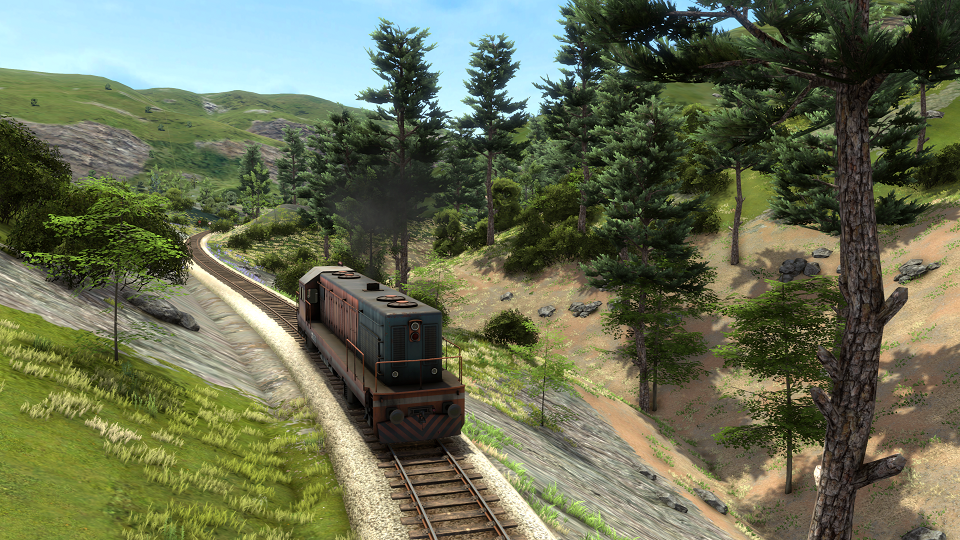
\includegraphics[width=9cm]{figures/derailvalley.png}
    %\vspace{-12pt}
    \caption{Derail Valley (Altfuture)}
\end{wrapfigure} 

Slobodan Stevic, CEO at \textit{Altfuture} and developer of \textit{Derail Valley}, explains they chose Unity “... because its VR support was better than that of other engines, back in 2016.” When asked which engine he believes is best suited for VR simulators, he adds “... it depends on the type of the simulator, its scope and style choice, as well as prior team experience.” 

\bigskip
\begin{wrapfigure}{l}{9cm}
    \vspace{12pt}
    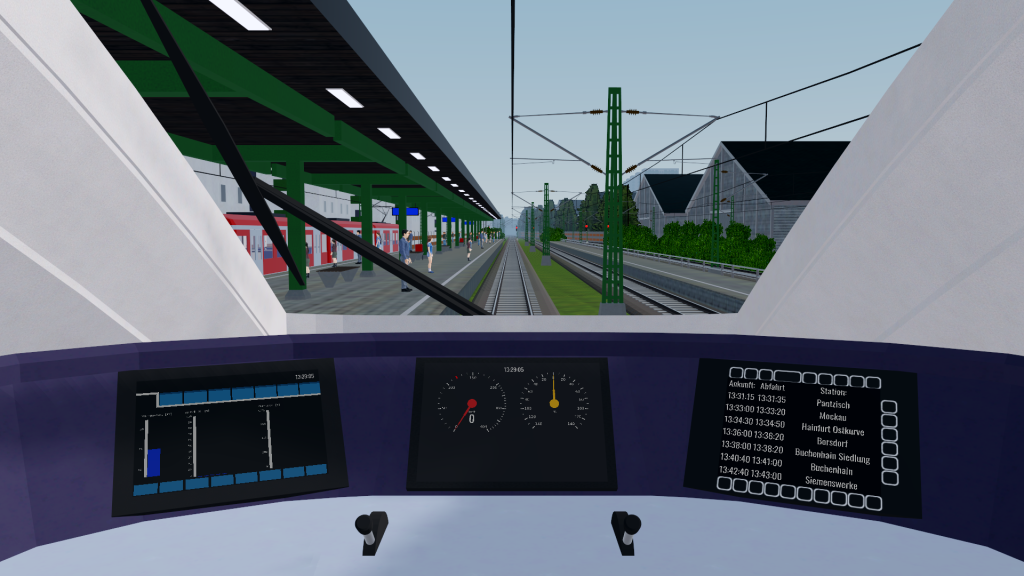
\includegraphics[width=9cm]{figures/libre_train_sim.png}
    %\vspace{-12pt}
    \caption{Libre TrainSim (GPL 3.0)}
\end{wrapfigure} 

Similarly, \textit{HaSa}, a contributor and developer of the open source project \textit{Libre TrainSim}, states that “as long as it supports `basic' requirements it is a matter of personal preference.” Describing the similarity of engine funnctioality, they also conclude that “the engine doesn't really matter.” \\[0.8cm]

Godot, the engine used to make Libre TrainSim, gets praised by HaSa for its agility. “Iteration speed is key to a good game in general. The more you iterate the better the result is.” They also comment on some downsides of the engine, claiming the renderer is “quite performance heavy out of the box which limits the creative freedom”, and the audio tools are `basic'. “We have to develop a lot of features on top to achieve good quality,” HaSa writes.

The developers we contacted behind CryEngine's small list of titles relevant to this analysis were unavailable for comment. When asking all subjects if they, in retrospect, believe their respective engine was the right choice for their game, everyone answered \textbf{yes}. 

%-----------------------------------------%

% todo
%%%                 Conclusion                  %%%
\section{Conclusion}
All engines, excluding Open 3D Engine, fulfills the Absolute Requirements (\ref{absoluterequirements}) set by Lokførerskolen. Godot and Unreal supports \texttt{gltf}-files, the most prioritized asset type. Meanwhile, CryEngine and Unity are at a disadvantage as they support fewer and less prioritized assets. While all engines require a conversion pipeline for assets, Unreal and Godot can reuse more assets out of the box. This decreases time spent on porting assets to the new engine.

The overall learning curve for the individual game engines sets Unity and Unreal engine apart from the competitors. The magnitude of the community and related quantity of available material, together with their emphasis on standards in documentation, establishes their strong position in today's game engine market. Godot is still a relatively new engine without any major titles, causing both documentation and community resources to be inadequate in quality and quantity compared to Unreal and Unity. CryEngine initially limited its use to enterprise only, resulting in less publicly available resources and documentation.

The majority of developers we reached out to advocated the choice of engine to depend on the use case of the project. As such we recommended Lokførerskolen to use Unreal Engine for their train simulator. Unreal Engine has features such as a built in dedicated spline tool which we ended up basing our whole train tracks system off, as well as dynamic occlusion culling to boost performance. It also has a one of the biggest communities among the engines analysed, as well as it is known for having photo-realistic graphics. Although finding the right solution to our problems was often an issue. We found that the community is split between using blueprints or C++, and often found that blueprints were most commonly used for beginners which slowed us down in the beginning. Since we started using blueprints first to prototype or solutions, and then later on converted it to C++ code.



%-------------------------------------------------------------------------------------------------

The \textit{jMonkeyEngine} game engine, currently in use by The Norwegian Train Driver Academy, has become primitive compared to modern technology. The importance and frequent usage of their train simulator inspire the need to migrate their software to a modern game engine. To mitigate this concern, several available solutions must be considered and evaluated.

All engines, excluding Open 3D Engine, fulfills the Absolute Requirements (\ref{absoluterequirements}) set by Lokførerskolen. Godot and Unreal supports \texttt{gltf}-files, the most prioritized asset type. Meanwhile, CryEngine and Unity are at a disadvantage as they support fewer and less prioritized assets. While all engines require a conversion pipeline for assets, Unreal and Godot can reuse more assets out of the box. This decreases time spent on porting assets to the new engine. 

The client being experienced with programming eliminates the need for GDScript as its most significant trait is being beginner-friendly. C\texttt{++}, on the other hand, may be unnecessarily advanced for the project. As for C\texttt{\#}, because of its powerful and modern functionality and versatile usage across game engines, we fail to see any relevant downsides, and we conclude it as a fitting language for the project.

The overall learning curve for the individual game engines sets Unity and Unreal engine apart from the competitors. The magnitude of the community and related quantity of available material, together with their emphasis on standards in documentation, establishes their strong position in today's game engine market. Godot is still a relatively new engine without any major titles, causing both documentation and community resources to be inadequate in quality and quantity compared to Unreal and Unity. CryEngine initially limited its use to enterprise only, resulting in less publicly available resources and documentation. 

The majority of the developers we reached out to advocated the choice of engine to heavily depend on the use case of the project. When developing an open world train simulator, this favors Unreal Engine as their engine provides tools such as dynamic occlusion culling, a dedicated spline tool and frequent release of tools used for in-house games.

In conclusion, we believe all four engines are capable of producing virtually any type of game. The difference lies in time and effort needed to achieve the same result. Throughout the analysis it is evident that Unity and Unreal Engine comes out as superior candidates, and would both be beneficial for this project. Despite Unreal Engine's steeper learning curve, we must consider the functionality provided for the specific use case of the project. Based on the results of this analysis, we conclude by proposing \textbf{Unreal Engine} to be the most suited solution for the mitigation of the current simulator.


% This here laid foundation for Requirements 
% Smooth transition to requirement specification - Henrik :D